\acf{top} is a new programming paradigm used to develop online collaborative applications. In a \acs{top} application, users --- both people and other systems --- work together to accomplish a common goal~\cite{top}. Its central concept is called a Task, an abstraction that can be used for many different types of work. This abstraction, along with other TOP concepts, allows the programmer to focus on design decisions instead of technical details. TOP programs are declarative: they focus on \textit{what} work should be performed, rather than on \textit{how} to perform it.

\section{iTasks}\label{itasks}
iTasks is an \acs{edsl} that implements the \acs{top} paradigm. Its host language is the pure and lazy functional programming language \textit{Clean}~\cite{clean}. iTasks uses generic programming to automatically generate code for user-specified first-order data types whilst also allowing for specialization. Given an iTasks program, the system generates code for both the server and the client.

An iTasks Task is a function that consumes a state and returns a \texttt{TaskValue} of type \texttt{a}, where \texttt{a} is the type of the task (represented by \texttt{Task a}). A \texttt{TaskValue} contains the current state of the value that a Task is processing. The possible states of a \texttt{TaskValue} are shown on Figure \ref{fig:task_value}. As we can see below, once a value stabilizes, it can not become unstable.


\begin{figure}[H]
\begin{center}
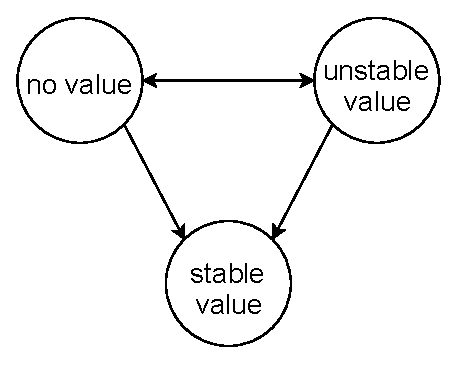
\includegraphics[scale=0.7]{thesis/img/task_value.eps}
\end{center}
\caption{Possible states of a \texttt{TaskValue}}
\label{fig:task_value}
\end{figure}

A Task can be of any type, as long as it provides instances for the type classes in the \texttt{iTask} type class collection. This instance can be automatically derived or explicitly declared. Automatic derivation is available for any type as long as it is not an abstract, extendable or the function type. Basic types have instances already defined in the iTasks library. Explicit declaration allows the user to define custom instances of the \texttt{iTask} class collection if the default derived instance is not suitable. Moreover, it allows instances for extendable, abstract and the function types. 

\section{Interaction}\label{interaction}

The iTasks library provides basic tasks for user interaction. Listing \ref{l_top1} shows the three basic interactive tasks: \texttt{enterInformation}, \texttt{viewInformation} and \texttt{updateInformation}. They create user interface elements to enter, view and update information respectively. As we can see in Listing \ref{l_top1}, these basic tasks include a class constraint on the type of the returned \texttt{Task}. This constraint enforces that the type \texttt{m} implements an instance of the \texttt{iTask} type class. 

\begin{lstlisting}[caption=iTasks basic interaction functions,captionpos=b,label=l_top1]
enterInformation  :: d [EnterOption m]      -> Task m | toPrompt d & iTask m
viewInformation   :: d [ViewOption m] m     -> Task m | toPrompt d & iTask m
updateInformation :: d [UpdateOption m m] m -> Task m | toPrompt d & iTask m 
\end{lstlisting}


Listing \ref{l_top2} displays examples of how to use the basic interactive tasks. We introduce a new \ac{adt}, called \texttt{Location} and automatically derive its instance of the \texttt{iTask} type class. Following, we introduce a new example \texttt{Location}. Finally, we define new tasks in terms of the basic tasks presented in Listing \ref{l_top1}. Here, keep in mind that the iTasks standard library implements an instance of the \texttt{toPromt} type class for the type \texttt{String}.  


\begin{lstlisting}[caption=Example of basic iTasks interaction functions,captionpos=b,label=l_top2]
:: Location = { city :: String, state :: String }

derive class iTask Location

location :: Location
location = { city="Omaha", state="Nebraska"}

enterLocation :: Task Location
enterLocation = enterInformation "Enter the location" []

viewLocation :: Task Location
viewLocation = viewInformation "View the location" [] location

updateLocation :: Task Location
updateLocation = updateInformation "Update the location" [] location
\end{lstlisting}

Figure \ref{fig:itasks_display} displays the user interfaces generated for the basic tasks \texttt{enterInformation} (Figure \ref{fig:enter_info}), \texttt{viewInformation} (Figure \ref{fig:view_info}) and \texttt{updateInformation} (Figure \ref{fig:upd_info}).

\begin{figure}[H]
\begin{subfigure}{0.33\textwidth}
\includegraphics[scale=0.7]{thesis/img/enter_location.png}
\caption{Enter Information}
\label{fig:enter_info}
\end{subfigure}
\begin{subfigure}{0.33\textwidth}
\includegraphics[scale=0.55]{thesis/img/view_location.png}
\caption{View Information}
\label{fig:view_info}
\end{subfigure}
\begin{subfigure}{0.33\textwidth}
\includegraphics[scale=0.7]{thesis/img/update_location.png}
\caption{Update Information}
\label{fig:upd_info}
\end{subfigure}
\caption{The visual representation of the basic iTasks interaction functions}
\label{fig:itasks_display}
\end{figure}


\section{Combinators}\label{combinators}

Although the basic tasks introduced in Section \ref{interaction} allow the user to exchange information with the iTasks application, they are quite limited. In order to allow the user to express more complex behavior, task combinators were introduced. Combinators are functions (usually infix operators) that determine how its argument tasks will be combined into a new task. There are only two fundamental composition combinators: sequence and parallel~\cite{top_fl}. All the other combinators in the \texttt{iTask} library are derived from these fundamental combinators. Only the derived combinators will be discussed in this document.

\subsection{Sequential Combinators}

Tasks can be executed in sequence using the \texttt{>>*} combinator, also called the \textit{step} combinator. Its type signature can been seen on Listing \ref{seq_comb}. The step combinator takes a \texttt{Task a} and a list of task continuations as input. A task continuation defines a condition on when to execute another task. It is a predicate that runs on either user actions, task values or thrown exceptions.

\begin{lstlisting}[caption=Sequential Combinators,label=seq_comb,captionpos=b]
(>>*) infixl 1 :: (Task a) [TaskCont a (Task b)] -> Task b | iTask a & iTask b

:: TaskCont a b                               
	= OnValue ((TaskValue a) -> Maybe b)         
	| OnAction Action ((TaskValue a) -> Maybe b) 
	| E.e: OnException (e -> b) & iTask e        
	| OnAllExceptions (String -> b)

(>>=) infixl 1 :: (m a) (a -> m b) -> m b   | iTask a & iTask b
(>>|) infixl 1 :: (m a) (m b)     -> m b   | iTask a & iTask b
\end{lstlisting}

The \texttt{>>=} (also called \textit{bind}) is an example of sequential combinator derived from the step combinator. Its first argument is the first task to be executed and its second arguments is a function that takes the first task's value as input and returns a task. The \texttt{>>|} combinator is derived from the bind combinator. It executes two tasks sequentially, but the value of the first task is disregarded. On both \texttt{>>=} and \texttt{>>|}, the second task is executed if either the value of the first task becomes stable, or it is unstable and the user presses a "Continue" button.

\subsection{Parallel Combinators}

Tasks can be executed in parallel using either the \texttt{-\&\&-} or the \texttt{-||-} combinators. The first executes two tasks in parallel and returns a tuple containing the result of both argument tasks. The \texttt{-||-} combinator executes two tasks in parallel and returns the task value of the first stable argument task. The type signatures of both combinators can be seen on Listing \ref{par_comb}.

\begin{lstlisting}[caption=Parallel Combinators,label=par_comb,captionpos=b]
(-||-) infixr 3 :: (Task a) (Task a) -> Task a     | iTask a
(-&&-) infixr 4 :: (Task a) (Task b) -> Task (a,b) | iTask a & iTask b
\end{lstlisting}


\section{Shared Data Sources}

Albeit task combinators are a powerful tool to 
communicate values among tasks, some applications often need to perform ad hoc communication with the external world. \acp{sds} abstract from implementation details on how resources are accessed. A resource can be, for example, a database, a file, the system time or a shared value in memory. 

Besides typed reading and writing, \acp{sds} provide a publish-subscribe system. If a task is observing an \ac{sds} that had been modified, the task is automatically notified on the change. This system allows for tasks to maintain up-to-date data without the need to constantly inspect the \ac{sds} for changes.

As it can be seen from Listing \ref{sds1}, an \texttt{SDS} has three type parameters. The first one is the type of the parametric lenses used on the notification system~\cite{parametric}. The second and third types are the read and write data types respectively. Note that they do not need to be the same type. A \texttt{ReadWriteShared} is an \ac{sds} where the parametric lens is of type \texttt{()} (void). As a consequence, a change in the shared will trigger all the tasks watching it. A \texttt{Shared} is a \texttt{ReadWriteShared} where read and write types are the same.

% SDS functions
There are four basic functions to operate on shares: \textit{get}, \textit{set}, \textit{update} and \textit{watch}. Their type signatures can be seen on Listing \ref{sds1}. The \texttt{get} operation simply fetches the current value of a share. Analogously, the \texttt{set} function sets a share's value. The \texttt{upd} operation sets a share's value based on its current value. The \texttt{watch} function waits for a notification of change from the share.

\begin{lstlisting}[caption=Shared Data Sources definitions,label=sds1,captionpos=b]
:: SDS p r w = ...
:: ReadWriteShared r w :== SDS () r w
:: Shared a :== SDS () a a

get   :: (ReadWriteShared a w)           -> Task a | iTask a
set   :: a (ReadWriteShared r a)         -> Task a | iTask a & TC r
upd   :: (r -> w) (ReadWriteShared r w)   -> Task w | iTask r & iTask w
watch :: (ReadWriteShared r w)           -> Task r | iTask r
\end{lstlisting}

\acp{sds} can be composed to create new \acp{sds} using combinators defined in the iTasks library. In addition, interactive tasks equivalent to the ones described in Section \ref{interaction} are defined for \acp{sds}. 